\smalltitle{سوال 1}
\begin{enumerate}
    \item پنج متغیر تعریف می‌کنیم که چهارتای اول برای مسئول هر تمرین است و آخری برای مسئول کل تمرین‌ها
    \begin{gather*}
        X = \{HW1, HW2, HW3, HW4, HW5, Head\}\\
        D = \{1, 2, 3, 4\}\\
        C = \{Lead \neq \{HW1, HW2, HW3, HW4, HW5\},\\
        HW2 \ne HW1, HW2 \ne HW3, HW4 \ne HW3, HW4 \ne HW5,\\
        HW1 \in \{1, 3, 4\}, HW2 \in {3, 4}, HW3 \in \{4\}, HW4 \in \{1, 2, 4\}, HW5 \in \{1, 2, 4\}
        \}
    \end{gather*}
    \begin{center}
        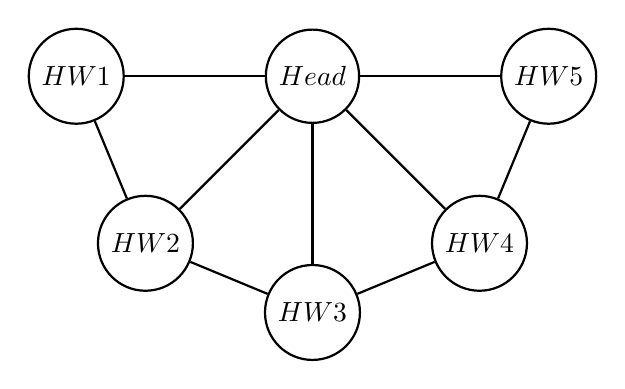
\begin{tikzpicture}[node distance={30mm}, thick, main/.style = {draw, circle}] 
            \node[main] (1) {$Head$};
            \node[main] (2) [left of=1] {$HW1$}; 
            \node[main] (3) [below left of=1] {$HW2$}; 
            \node[main] (4) [below of=1] {$HW3$}; 
            \node[main] (5) [below right of=1] {$HW4$}; 
            \node[main] (6) [right of=1] {$HW5$}; 

            \draw[-] (1) -- node[midway, above, sloped] {} (2);
            \draw[-] (1) -- node[midway, above, sloped] {} (3);
            \draw[-] (1) -- node[midway, above, sloped] {} (4);
            \draw[-] (1) -- node[midway, above, sloped] {} (5);
            \draw[-] (1) -- node[midway, above, sloped] {} (6);

            \draw[-] (2) -- node[midway, above, sloped] {} (3);
            \draw[-] (3) -- node[midway, above, sloped] {} (4);
            \draw[-] (4) -- node[midway, above, sloped] {} (5);
            \draw[-] (5) -- node[midway, above, sloped] {} (6);
        \end{tikzpicture}
    \end{center}
    \item بله. کافی است که \lr{head} را مشخص کنیم.
    \item دقت کنید که TA چهارم را نمی‌توانیم هد کنیم چرا که در این صورت کسی کلا تمرین 3 را بر نمی‌دارد.
    تی‌ای شماره 3 هم نمی‌توانیم هد کنیم چرا که در این صورت در تمرین 2 و 3 به مشکل می‌خوریم و مجبور می‌شویم که شماره 4
    را به آنها \lr{assign} کنیم.
    حال بین بقیه‌ی \lr{TA}ها یک هد انتخاب می‌کنیم.

    حال برای حالاتی که نفر اول و دوم هد هست به ترتیب به کمک \lr{filter} و \lr{order} سعی می‌کنیم که مسئله را حل کنیم.
    \begin{gather*}
        X_1 = \{\_,\_,\_,\_,\_,1\} \rightarrow \{\_,\_,4,\_,\_,1\} \rightarrow \{\_,3,4,\_,\_,1\} \rightarrow \{4,3,4,\_,\_,1\} \\
        \rightarrow \{4,3,4,2,\_,1\} \rightarrow \{4,3,4,2,4,1\}\\
        X_2 = \{\_,\_,\_,\_,\_,2\} \rightarrow \{\_,\_,4,\_,\_,2\} \rightarrow \{\_,3,4,\_,\_,2\} \rightarrow \{4,3,4,\_,\_,2\} \\
        \rightarrow \{4,3,4,1,4,2\} \rightarrow \{4,3,4,1,4,2\}
    \end{gather*}
\end{enumerate}








